\documentclass{sintefbeamer}

% packages, font, color, and newcommands
\usepackage{amsfonts, amsmath, oldgerm, lmodern, bm}
% \usepackage[font={footnotesize}]{caption}
\usepackage{natbib}
\usepackage{url}
\usepackage{tikz}
\usepackage{amssymb}
\usepackage{amsmath}
\usepackage{amsthm}
\usepackage{mathrsfs}
\usepackage{empheq}
\usepackage{mdframed}
\usepackage{bm}
\usepackage{animate}
\usepackage{xcolor,colortbl}
\usepackage{graphicx}
\bibliographystyle{apalike}
\usefonttheme{serif}
\usetikzlibrary{calc}
\definecolor{carminered}{rgb}{1.0, 0.0, 0.22}
\definecolor{burgundy}{rgb}{0.5, 0.0, 0.13}
\title{Averaged equations for mono-disperse two-phase flows made of non-spherical particles. }
\subtitle{MUSCATS workshop}
\author{\underline{N. Fintzi} \footnote{IFP \'Energies Nouvelles, France}$^{,2}$, JL. Pierson$^1$ and D. Lhuillier\footnote{Sorbonne Universit\'e, France}}
% \date{Created on May 22, 2022}
\definecolor{burntorange}{rgb}{0.8, 0.33, 0.0}
\titlebackground{../../CYLINDERS_PROJECT/RoadToJFM/image/cyl.png}

% document body
\addtobeamertemplate{navigation symbols}{}{%
    \usebeamerfont{footline}%
    \usebeamercolor[fg]{footline}%
    % \hspace{1em}%
    % \vspace{1em}%
    \insertframenumber/\inserttotalframenumber
}
\usepackage{stmaryrd}


\begin{document}
\maketitle
\section*{}

\begin{frame}
  \frametitle{Objectives}

In the perspective of \textbf{Euler-Euler} framework modeling we : 
\begin{enumerate}
  \item Demonstrate how to derive the \textbf{mass} and \textbf{momentum} averaged equations for non-spherical particle suspension. 
  \begin{itemize}
    \item The dispersed phase is averaged using a kinetic theory-like approach \citep{jackson1997locally,zhang1994averaged}
    \item The fluid phase is averaged following the classic average method \citep{drew1983mathematical}. 
  \end{itemize}
  % \item Discus the implication of having spheroidal particles in opposition to spherical particles. 
  %   \begin{itemize}
  %     \item How to derive an equation for the orientation.
  %     \item How to derive an equation for the angular momentum.
  %   \end{itemize}
  \item Show how it is related to the carrier phase equations.  
  % \item What is the expression of the particle and fluid equivalent stress ?
\end{enumerate}
\end{frame}

\section{Derivation of the fluid phase averaged equations.}
\section*{}

\begin{frame}
  \frametitle{Problem statement}

  \begin{figure}[h!]
    \centering
    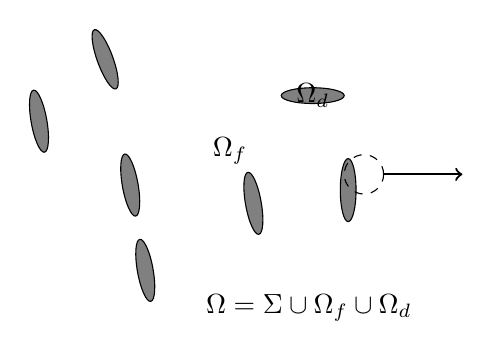
\begin{tikzpicture}
        \foreach \x/\y/\ra/\r/\th in 
        {1/3/0.4/0.1/20,
        2.55/2.7/0.1/0.4/0,
        0.5/0.4/0.4/0.1/10,
        2/1/0.4/0.1/10,
        3/1.5/0.4/0.1/0,
        0.5/1.5/0.4/0.1/10,
        -0.5/2.5/0.4/0.1/10}{
            \draw[fill=gray,rotate=\th](\x,\y) ellipse(\r cm and \ra cm);
        }
        \draw[dashed](3.2,1.7)circle(0.25);
        % \draw[thick,->](3.2,1.7)++(0.1767,0.1767)--++(0.4,0.4)--++(1,0);
        \draw[thick,->](3.2,1.7)++(0.25,0)--++(1,0);
        \draw(2.55,2.7)node{$\Omega_d$};
        \draw(1.5,2)node{$\Omega_f$};
        \draw(2.5,0)node{$\Omega = \Sigma \cup \Omega_f \cup \Omega_d$};
        % \draw(2.5,-1)node{$\Sigma = \sum_\alpha \Sigma_\alpha$};
        % \draw(2.5,-0.5)node{$\Omega_d = \sum_\alpha \Omega_\alpha$};
    \end{tikzpicture}
    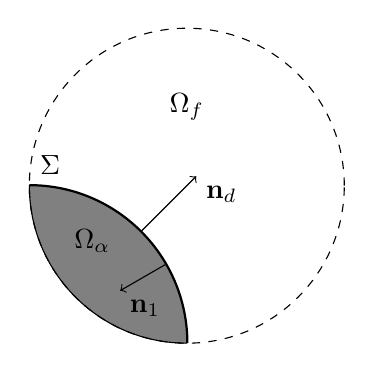
\begin{tikzpicture}%[scale = 0.9]
        \draw[very thick](0:2)arc(0:90:2)node[above right]{$\Sigma$};
        \draw[fill=gray](0:2)arc(0:90:2)arc(180:270:2);
        \draw[dashed](2,2)circle(2);
        \draw[->](1.42,1.42)--++(0.7,0.7)node[below right]{$\textbf{n}_d$};
        \draw[->](1.73,1)--++(-0.577,-0.333)node[below right]{$\textbf{n}_1$};
        \draw(2,3)node{$\Omega_f$};
        \draw(0.8,1.3)node{$\Omega_\alpha$};
    \end{tikzpicture}
    \caption{Domain definitions and scheme of the topology of dispersed two-phase flows.
    $\rho_k$ and $\mu_k$ is the density and viscosity of phase $k$, respectively. }
    \label{fig:Scheme}
\end{figure}

The phase and interface indicator functions : 
\begin{align*}
  \chi_k(\textbf{x},t) =  \left\{
    \begin{tabular}{cc}
      $1 \;\text{if} \;\textbf{x} \in \Omega_k(t)$\\
      $0 \;\text{if} \;\textbf{x} \notin \Omega_k(t)$
    \end{tabular}
    \right.
    % \text{for $k = 1,2$},
    % \label{eq:PIF}
    &&
  \delta_I(\textbf{x},t) =  \left\{
    \begin{tabular}{cc}
      $1 \;\text{if} \;\textbf{x} \in \Sigma(t)$\\
      $0 \;\text{if} \;\textbf{x} \notin \Sigma(t)$
    \end{tabular}
    \right.,
    \label{eq:PIF_I}
\end{align*}

\end{frame}



\begin{frame}
  \frametitle{Local scale mass and momentum laws.}
  The mass $\rho_k$ and momentum $\rho_k \textbf{u}_k^0$, conservation in the volumes follow :
\begin{align}
  \div  \textbf{u}_k^0
  &= 
  0
  \;\;\;\; 
  \text{in} 
  \;\;\;\; 
  \Omega_k(t)\\
  \pddt (\rho_k \textbf{u}_k^0)  
  + \div (
      \rho_k \textbf{u}_k^0\textbf{u}_k^0
      - \bm{\sigma}_k^0 
      )
  &= 
  \rho_k \textbf{g}
  \;\;\;\; 
  \text{in} 
  \;\;\;\; 
  \Omega_k(t)
\end{align}
And at the interfaces : 
\begin{align*}
  \Jump {\textbf{u}_k^0}
  = 0,\;\;\;
  \Jump {\bm{\sigma}_k^0}
  = 
  %  \gamma\kappa\textbf{n}
  0
   \;\;\;\; 
   \text{at} 
   \;\;\;\; 
   \Sigma(t)
\end{align*}
\begin{definition}
  \begin{itemize}
    \item $\Jump{\ldots} = \sum_k \ldots$ Jump condition.  
    \item The superscript $^0$ indicated that it is a local quantity.
    \item $\rho_k$  density of phase $k$. 
    \item $\textbf{u}_k$  Velocity of phase $k$.
    \item $\textbf{b}_k^0 = \rho_k \textbf{g}$  local body force.  
    \item $\gamma$ and $\kappa$  surface tension coefficient and curvature of the surface.  
    \item $\bm\sigma_f^0 = -p_f^0 \textbf{I} + \mu_f (\grad \textbf{u}_f^0+^\dagger\grad \textbf{u}_f^0)$ Newtonian stress tensor of the fluid phase. 
    \item $\bm\sigma_d^0 = \textbf{Udefined}$ Solid phase stress. 
  \end{itemize}
\end{definition}

\end{frame}


% \begin{frame}
%   \frametitle{Two-fluid formulation of the momentum equation.}
% %   Transport of the phase indicator function, 
% %   \begin{align}
% %     \pddt \chi_k
% %     + \textbf{u}_I^0 \cdot \grad \chi_k
% %     = 0,&&
% % % \end{align}
% % % \begin{align}
% %     \grad \chi_k
% %     = - \delta_I \textbf{n}_k
% %   \end{align}
%   Multiplying the momentum equation by $\chi_k$ gives two-fluid formulation of the momentum equation :
  
%   \begin{align}
%     \label{eq:mass}
%     \pddt (\chi_k\rho_k)  
%     + \div (
%         \chi_k\rho_k \textbf{u}_k^0
%         )
%     &= 0\\
%     \pddt (\chi_k\rho_k \textbf{u}_k^0)  
%     + \div (
%         \chi_k\rho_k \textbf{u}_k^0\textbf{u}_k^0
%         - \chi_k\bm{\sigma}_k^0 
%         )
%     &= 
%     \chi_k\textbf{b}_k^0
%     + \underbrace{\delta_I \bm{\sigma}_k^0\cdot\textbf{n}_k}_\text{Interphase momentum transfer}
%     \label{eq:momentim}
%   \end{align}

%   $\to$ notice that (\ref{eq:mass}) and (\ref{eq:momentim}) are defined over $\Omega$ thanks to $\chi_k$. 
%   Therefore, we are now able to apply the ensemble average procedure. 
% \end{frame}


\begin{frame}
  \frametitle{Ensemble average definition}
%   Let, $P(\FF)$ be the probability density function that describe the probability of finding the flow in the configuration $\FF$, were $\FF = (\lambda_1,\lambda_d,\lambda_3,\ldots)$ is a finite set of all the parameters describing the initial flow configuration.
% \footnote{Assuming that the flow can be described by a finite number of parameters related to both phase...}. 
% We define $d\mathscr{P} = P(\FF)d\FF$ as the probable number of flow in the incremental region of the particles' phase space $d\FF$ around $\FF$. 
% It follows from this definition, that the ensemble average of an arbitrary local property $f^0[\textbf{x},t;\FF]$ defined on the whole space $\Omega$, is,
The continuous and particle ensemble  averaged energy : 
\begin{align*}
  \phi_k (\textbf{x},t) = \avg{\chi_k }\\
  \phi_k \rho_k  \textbf{u}_k (\textbf{x},t) = \avg{\chi_k \rho_k \textbf{u}_k^0 }\\
  \phi_k \bm\sigma_k (\textbf{x},t) = \avg{\chi_k \bm\sigma_k^0 }\\
  % \phi_k \textbf{b}_k (\textbf{x},t) = \avg{\chi_k \textbf{b}_k^0 }
  \label{eq:1_avg}
\end{align*}
% \begin{equation}
%   n_p E_p(\textbf{x},t) = \avg{\sum_\alpha^N \delta(\textbf{x} - \textbf{x}_\alpha(\FF,t)) E_\alpha}
%   \label{eq:p_avg}
% \end{equation}
\begin{definition}
  \begin{itemize}
    \item $\avg{\ldots}$ ensemble average operator. 
    \item  $\phi_k (\textbf{x},t)$ volume fraction of the phase $k$. 
    \item Note that we dropped the superscript $^0$ on $\textbf{u}^0_k$ to indicate that $\textbf{u}_k$ is a macroscopic quantity. 
    % \item $n_p (\textbf{x},t) = \avg{\sum_\alpha^N \delta(\textbf{x} - \textbf{x}_\alpha(\FF,t))}$ number density of particles. 
    % \item  Both are linked through :   $\phi_d \rho_d= m_p n_p + \frac{1}{2}\grad^2 : (n_p\mathcal{M}_p)+\ldots$
  \end{itemize}
\end{definition}
\end{frame}

\begin{frame}
  \frametitle{The averaged two-fluid model }
\begin{align*}
  \phi_d + \phi_f &= 1\\
  \pddt (\phi_k \rho_k)  
  + \div (\phi_k \rho_k\textbf{u}_k)
  &= 
  0\\
  \pddt (\phi_k \rho_k\textbf{u}_k)  
  + \div (
      \phi_k \rho_k\textbf{u}_k\textbf{u}_k
      + \bm{\sigma}_k^\text{eq}
  )
  &= 
  \phi_k  \rho_k \textbf{g}
  +  \avg{\delta_I \bm{\sigma}_k^0 \cdot \textbf{n}_k}
\end{align*}
with, 
\begin{align*}
  &\bm{\sigma}_k^\text{eq}
  = 
   \underbrace{\rho_k\avg{\chi_k \textbf{u}_k'\textbf{u}_k'}}_\text{Reynolds stress}
    - \phi_k \bm{\sigma}_k,%- n_p \textbf{M}_p
\end{align*}
\textbf{Problems on the two-fluid model : }
\begin{enumerate}
  \item $\avg{\delta_I \bm{\sigma}_k^0 \cdot \textbf{n}_k} =f(Re,\phi,\text{particles' propreties})$
  \item Is the dispersed phase stress $\bm\sigma_d$, really able to have a role in the momentum balance of the particles ? 
  \item  Why the two-fluid model has no consideration for the angular momentum of the particles ? 
\end{enumerate}

\end{frame}


\section{Derivation of the particle phase averaged equation.}
\section*{}


\begin{frame}
  \frametitle{Particles's degrees of freedom}
  \begin{columns}
    \column{0.2\textwidth}
    \begin{figure}[h!]
      \centering
      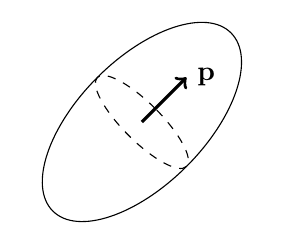
\begin{tikzpicture}[rotate=45,scale = 0.8]
        \draw(0,0) ellipse (2 cm and 1 cm);
        \draw[dashed](0,0) ellipse (0.3 cm and 1 cm);
        \draw[->,very thick](0,0) --++ (1,0)node[right]{$\textbf{p}$};
      \end{tikzpicture}
      \caption{Scheme of an axis symmetric particle with fore after symmetry and orientation vector \textbf{p}.}
    \end{figure}
    \column{0.8\textwidth}
\textbf{Particles properties :}
\begin{itemize}
  \item $m_\alpha$ mass 
  \item $\textbf{p}$ orientation vector.  
  \item $\textbf{u}_\alpha$ Particle's velocity 
  \item $\bm\omega_\alpha$ angular velocity pseudo vector. 
\end{itemize}

$\to$ The particle has 10 degree of freedom  ($\textbf{u}_\alpha(3) + \textbf{p}(3) + \bm\Omega_\alpha (3) + m_\alpha (1) = 10$), meaning that we need at least $10$ equations. 
\end{columns}

\end{frame}


\begin{frame}
  \frametitle{Mass, position and momentum of a single particle}


  We define the total volume mass and momentum the particle $\alpha$ by, 
  \begin{align*}
    m_\alpha(t)
    = \int_{\Omega_\alpha(t)} \rho_d d\textbf{x}
    &&
    \textbf{x}_\alpha(t)
    = \frac{1}{m_\alpha}\int_{\Omega_\alpha(t)} \rho_d \textbf{x} d\textbf{x}
    &&
    m_\alpha \textbf{u}_\alpha(t) 
    = \int_{\Omega_\alpha(t)} \rho_d \textbf{u}_d^0 d\textbf{x}
  \end{align*}
  \begin{align*}
    \textbf{M}_\alpha(t) 
    = \int_{\Omega_\alpha(t)} \rho_d \textbf{rr} d\textbf{x} &&
    \textbf{P}_\alpha(t) 
    = \int_{\Omega_\alpha(t)} \rho_d \textbf{r} \textbf{u}_d^0 d\textbf{x}
  \end{align*}
  \begin{definition}
    \begin{itemize}
      \item $ \Omega_\alpha(t)$ domain of the particle. 
      \item $ \textbf{x}_\alpha $ center of mass of the particle. 
      \item $\textbf{r} = \textbf{x} - \textbf{x}_\alpha(t)$ Relative position vector. 
      % \item $\textbf{w}_d^0 = \textbf{u}_d^0 - \textbf{u}_\alpha(t)$ Relative velocity vector with respect to the center of mass velocity. 
      \item $\textbf{M}_\alpha(t)$ Second moment of mass. 
      
      Note that $\textbf{M}_\alpha(t)$ is related to the inertia matrix $\textbf{I}_\alpha$ with : $\textbf{I}_\alpha = (\textbf{M}_\alpha : \textbf{I} )\textbf{I}- \textbf{M}_\alpha$
      \item $\textbf{P}_\alpha(t)$ First moment of momentum. 
      
      $\textbf{P}_\alpha$ is related to the angular momentum $\bm\mu_\alpha$ following $\bm\mu_\alpha =\bm\epsilon : \textbf{P}_\alpha$
    \end{itemize}
  \end{definition}

% \textcolor{red}{\textbf{Warning : } In the next slides we use the notations :  $\intO{\ldots} = \int_{\Omega_\alpha} \dots d\Omega$ and  $\intS{\ldots} = \int_{\Sigma_\alpha} \dots d\Sigma$.}
\end{frame}




\begin{frame}
  \frametitle{Particle conservation laws }
\begin{align*} 
  \text{Mass :   }
  &
  \ddt \intO{\rho_d}
  = 
  0\\
  \text{Momentum :   }
  &
  \ddt \intO{\rho_d \textbf{u}_d^0}
  = 
  \int_{\Omega_\alpha(t)} \rho_k \textbf{g} d\Omega  
  + \intS{\bm{\sigma}_f^0 \cdot \textbf{n}_d}
  \\
  \substack{\text{Second moment} \\ \text{of mass }} : 
  &
  \ddt \intO{\rho_d \textbf{rr}}
  = \intO{(\textbf{r} \textbf{u}_d^0+\textbf{u}_d^0\textbf{r} )}\\
  \substack{\text{First moment} \\ \text{of momentum }} : 
  &
  \ddt \intO{\textbf{ru}_d^0}
  = \intO{ \rho_d  \textbf{w}_d^0 \textbf{w}_d^0 }
  - \intO{\bm{\sigma}_d^0 }
  + \intS{ \textbf{r}\bm{\sigma}_f^0\cdot \textbf{n}_d}
\end{align*}
  
\begin{enumerate}
  \item These are valid for arbitrary particles without surface properties. 
  \item  We have 24 equations, it is too much for solid particles, let's proceed to some simplifications. 
\end{enumerate}

\end{frame}

\begin{frame}
  \frametitle{Internal velocity fields for a solid particles}
  For solid bodies with angular velocity $\bm\omega_\alpha$ we have,
  \begin{align*}
    \textbf{u}_d^0(\textbf{x}_\alpha + \textbf{r}) = 
    \textbf{u}_\alpha + \textbf{w}_d^0  = 
    \underbrace{\textbf{u}_\alpha(t)}_\text{center of mass velocity}
    + \underbrace{\textbf{r}\times \bm\omega_\alpha(t)}_\text{internal velocity}
  \end{align*}

  With this definition, the integrals in the previous equations read,
  \begin{align*}
    \int_{\Omega_\alpha(t)} \rho_d \textbf{r} \textbf{u}_d^0 d\textbf{x}
    = 
    \textbf{M}_\alpha \times \bm\omega_\alpha
    \\
    \int_{\Omega_\alpha(t)} \rho_d \textbf{w}_d^0 \textbf{w}_d^0 d\textbf{x}
    = \bm\omega_\alpha\times \textbf{M}_\alpha\times \bm\omega_\alpha
\end{align*}

% $\to$ Notice that the second moment of mass can be express with the orientation vector : $\mathbf{M}_\alpha = \textbf{pp} M_{||}+ \textbf{I} M_\bot$. 
% Remark :
\begin{enumerate}
  \item At this stage we could implement more sophisticated internal velocity fields if the particles were deformable.  
\end{enumerate}
\end{frame}

\begin{frame}
  \frametitle{The second moment of mass equation }
  \begin{equation*}
    \ddt \intO{\rho_d\textbf{rr}} =
    \ddt 
    \underbrace{\textbf{M}_\alpha}_\text{Particle distribution of mass}
    =
    \underbrace{\textbf{M}_\alpha \times \bm\omega_\alpha+ \bm\omega_\alpha \times \textbf{M}_\alpha }_\text{Particle rate of strain}
  \end{equation*}
  
  $\to$ Let, $\textbf{M}_\alpha = \textbf{pp} M_{||} + \textbf{I} M_\bot $ with $M_{||}$ and $M_\bot$ two constant related to the shape of the particles.
  Then the second moment of mass equation becomes an equation for the \textbf{orientation} such that, 
  \begin{equation}
    \ddt \textbf{pp} = 
    \bm\omega_\alpha \times \textbf{pp}
    + \textbf{pp} \times \bm\omega_\alpha.
  \end{equation}
  Or for the inertial martrix $\textbf{I}_\alpha = - \textbf{M}_\alpha + \frac{1}{2}(\textbf{M}_\alpha : \textbf{I})\textbf{I}$, we also have,
  \begin{equation}
    \ddt \textbf{I}_\alpha = 
    \bm\omega_\alpha \times \textbf{I}_\alpha
    + \textbf{I}_\alpha \times \bm\omega_\alpha.
  \end{equation}
  % Conclusions :
  \begin{enumerate}
    \item So solving either for $\textbf{M}_\alpha$, $\textbf{I}_\alpha$ or \textbf{pp} is basically the same thing.
    \item From these equations $1/\bm\omega_\alpha$ is the relaxation time of the orientation tensor. 
    \item This is the starting point of the Flogar-tucker equaitons. 
  \end{enumerate}
\end{frame}
\begin{frame}
  \frametitle{Skew-symmetric moment of momentum  equation }
  That is the moment of momentum equation :
\begin{equation*}
  \ddt (\textbf{M}_\alpha \times \bm\omega_\alpha)
  = \bm\omega_\alpha\times \textbf{M}_\alpha\times \bm\omega_\alpha
  - \intO{\bm{\sigma}_d^0 }
  + \intS{ \textbf{r}\bm{\sigma}_f^0\cdot \textbf{n}_d}
\end{equation*}

The \textbf{Skew-symmetric} part of the moment of momentum equation is,  
\begin{equation*}
  \ddt \bm\mu_\alpha
  = 
  \ddt \underbrace{\textbf{I}_\alpha \cdot \bm\omega_\alpha}_\text{Angular momentum}
  = 
  \underbrace{\intS{ \textbf{r} \times \bm{\sigma}_f^0\cdot \textbf{n}_d}}_\text{Hydrodynamic torque}
\end{equation*}
\begin{definition}
  \begin{itemize}
    \item  $\intO{\textbf{r} \times \textbf{u}_d^0} = \textbf{I}_\alpha \cdot \bm\omega_\alpha = \bm\mu_\alpha$, Angular momentum various notations. 
  \end{itemize}
\end{definition}
\end{frame}

\begin{frame}
  \frametitle{The particle stress equation }
  

The \textbf{symmetric} part of the moment of momentum equation can be view as an equation for the \textbf{internal stress} (assuming the internal stress is symmetric),  
\begin{equation*}
  \underbrace{\intO{\bm{\sigma}_d^0 }}_\text{Internal stress}
  = \underbrace{\bm\omega_\alpha\times\textbf{M}_\alpha\times\bm\omega_\alpha}_\text{Internal velocity}
  - \ddt \underbrace{(\textbf{M}_\alpha \times \bm\omega_\alpha+ \bm\omega_\alpha \times \textbf{M}_\alpha)}_\text{Rate of strain derivative}
  + \underbrace{\intS{ (\textbf{r}\bm{\sigma}_f^0+\bm{\sigma}_f^0\textbf{r})\cdot \textbf{n}_d}}_\text{Stresslet}
  \label{eq:dt_P_alpha}
\end{equation*}

% \textbf{Conclusions : }
\begin{enumerate}
  \item The \textbf{skew-symmetric} part of the moment of momentum equation is the angular momentum conservation. 
  \item The \textbf{symmetric} part of the moment of momentum equation is an equation  for the particle internal stress, assuming we already solve for, $\bm\omega_\alpha$, $\textbf{I}_\alpha$, and upon having an expression for the stresslet such that : $\intS{ (\textbf{r}\bm{\sigma}_f^0+\bm{\sigma}_f^0\textbf{r})\cdot \textbf{n}_d} = f(\textbf{u}_\alpha, \textbf{M}_\alpha,\bm\omega_\alpha)$ , 
  \item For \textbf{deformable particles} it would have been an equation for the \textit{Rate of strain}. 
\end{enumerate}



\end{frame}



\begin{frame}
  \frametitle{Particle conservation laws }
\begin{align*} 
  \text{Mass :   }
  &
  \ddt m_\alpha
  = 
  0\\
  \text{Momentum :   }
  &
  \ddt (m_\alpha \textbf{u}_\alpha )
  = 
  m_\alpha \textbf{g}  
  + \intS{\bm{\sigma}_f^0 \cdot \textbf{n}_d}
  \\
  \substack{\text{Second moment} \\ \text{of mass }} : 
  &
  \ddt \textbf{I}_\alpha
  = \textbf{I}_\alpha \times \bm\omega_\alpha+ \bm\omega_\alpha \times \textbf{I}_\alpha \\
  \substack{\text{Angular moment} \\ \text{of momentum }} : 
  &
  \ddt \bm\mu_\alpha
  =  
  \intS{ \textbf{r}\times\bm{\sigma}_f^0\cdot \textbf{n}_d}
  \\
  \substack{\text{Stress} \\ \text{equation}} : 
  &
  \intO{\bm{\sigma}_d^0 }
  =  \bm\omega_\alpha \times \textbf{M}_\alpha\times \bm\omega_\alpha
  - \ddt^2 \textbf{I}_\alpha
  + \intS{( \bm{\sigma}_f^0 \textbf{r}+  \textbf{r}\bm{\sigma}_f^0) \cdot \textbf{n}_d}
\end{align*}
  
% Conclusion :
\begin{enumerate}
  \item We have only $2$ closure in the system : 
  \begin{itemize}
    \item The external momentum flux / drag force : 
    $\intS{\bm{\sigma}_f^0 \cdot \textbf{n}_d}$
    \item The first moment of the external momentum flu : 
    $\intS{ \textbf{r}\bm{\sigma}_f^0\cdot \textbf{n}_d}$
  \end{itemize}
  \item And 3 unknown, $\textbf{u}_\alpha$,$\textbf{I}_\alpha$ and $\bm\omega_\alpha$.
\end{enumerate}


\end{frame}


\section{Particle phase averaged equations}
\section*{}

\begin{frame}
  \frametitle{Particle ensemble average definition}
The  \textit{particle} ensemble  average is defined as : 
\begin{align*}
  \text{Number density : }\;\;\;&
  n_p (\textbf{x},t) =  \pavg{ }\\
  \text{Averaged particle velocity : }\;\;\;&
  n_p \textbf{u}_p(\textbf{x},t) =  \pavg{  \textbf{u}_\alpha}\\
  \text{Averaged particle orientation : }\;\;\;&
  n_p \textbf{I}_p(\textbf{x},t) =  \pavg{  \textbf{I}_\alpha}\\
  \text{Averaged angular velocity  : }\;\;\;&
  n_p \bm\omega_p(\textbf{x},t) 
  =  
  \pavg{  \bm\omega_\alpha}\\
  \text{Averaged angular momentum  : }\;\;\;&
  n_p \bm\mu_p(\textbf{x},t) =  
  \bm\omega_p \cdot \textbf{I}_p
  + \pavg{  \bm\omega_\alpha'\cdot \textbf{I}_\alpha'} \\
  \text{Averaged first moment of momentum  : }\;\;\;&
  n_p \textbf P_p(\textbf{x},t) =  
  \bm\omega_p \times \textbf{I}_p
  + \pavg{  \bm\omega_\alpha'\times \textbf{I}_\alpha'} \\
\end{align*}
\begin{definition}
  \begin{itemize}
    \item $\delta_\alpha = \sum_\alpha \delta(\textbf{x} - \textbf{x}_\alpha(\FF,t))$ Is the particle phase indicator function, which is non-zero at the center of mass of the particles. 
  \end{itemize}
\end{definition}

\begin{enumerate}
  \item The total angular momentum of the dispersed phase actually contain a fluctuation terms, that we will note : $\textbf k^{\bm\omega \textbf{I}} = \pavg{  \bm\omega_\alpha' \textbf{I}_\alpha'} $
  \item Thus, the averaged angular momentum might be non-zero while $\bm\omega_p = 0$.
\end{enumerate}
\end{frame}

\begin{frame}
  \frametitle{Averaged particle's phase equations}
Applying the average operator directly gives the \textbf{primary}  equations, 
  \begin{align*} 
    \text{Mass :   }
    &
    \pddt n_p + \div (\textbf{u}_p n_p)
    = 
    0\\
    \text{Momentum :   }
    &
    \pddt (n_p\textbf{u}_p) + \div (\textbf{u}_p\textbf{u}_p n_p+ \textbf{u}^\text{Re}_p)
    = 
    n_pm_p\textbf{g}
    + \pavg{\intS{\bm{\sigma}_f^0 \cdot \textbf{n}_d}}
    \\
    \substack{\text{Second moment} \\ \text{of mass }} : 
    &
    \pddt (\textbf{I}_p n_p )+ \div (\textbf{I}_p\textbf{u}_p  n_p + \textbf{I}^\text{Re}_p)
    = \textbf{I}_p \times \bm\omega_p+ \bm\omega_p \times \textbf{I}_p + 2\bm\epsilon : \textbf{k}^{\bm\omega \textbf{I}}\\
    \substack{\text{Angular  moment} \\ \text{of momentum }} : 
    &
    \pddt (\bm\mu_p n_p)+ \div (\bm\mu_p \textbf{u}_p  n_p + \bm\omega_p\cdot\textbf{I}^\text{Re}_p + \bm\mu_p^\text{Re})
    =  
     \pavg{\intS{ \textbf{r}\times\bm{\sigma}_f^0\cdot \textbf{n}_d}}
    % \substack{\text{Particle stress} \\ \text{equation }} : 
    % &
    % \pOavg{\bm{\sigma}_d^0 }
    % =  \pavg{\bm\omega_\alpha \times \textbf{M}_\alpha \times \bm\omega_\alpha}
    % - \pavg{\ddt (\bm\omega_\alpha \times \textbf{M}_\alpha )}
    % + \pSavg{ \textbf{r}\bm{\sigma}_f^0 \cdot \textbf{n}_d}
  \end{align*}

  The fluctuation closure terms : 
  \begin{align*}
    n_p \textbf{u}_{p}^\text{Re}
    % n_p \textbf{k}_{p}^{\textbf{I}\textbf{u}}
    % = 
    =
    \pavg{\textbf{u}_\alpha' \textbf{u}_{\alpha}'}
    &&
    n_p \textbf{I}_{p}^\text{Re}
    % n_p \textbf{k}_{p}^{\textbf{I}\textbf{u}}
    % = 
    =
    \pavg{\textbf{I}_\alpha' \textbf{u}_{\alpha}'}
    &&
    n_p \bm\mu_{p}^\text{Re}
    = 
    \pavg{\textbf{I}'_\alpha\cdot \bm\omega'_\alpha \textbf{u}_\alpha'} 
    + \textbf{I}_p \cdot \pavg{\bm\omega_\alpha' \textbf{u}_\alpha'}
\end{align*}
\begin{enumerate}
  \item Four equations for four unknowns, ( $n_p, \textbf{u}_p, \bm\omega_p$ and $\textbf{I}_p$), if we omit the closure terms. 
\end{enumerate}
\end{frame}


\begin{frame}
  \frametitle{Second form of the angular momentum equation}
Dot product the equation for $\textbf{I}_p$ with $\bm\omega_p$ yields, 
\begin{multline}
    \pddt (\bm\omega_p \cdot \textbf{I}_p n_p )+ \div (\bm\omega_p\cdot \textbf{I}_p\textbf{u}_p  n_p + \omega_p\cdot \textbf{I}^\text{Re}_p\cdot )
    = 
    \textbf{I}_p^\text{Re} : \grad\bm\omega_p
    + \bm\omega_p\cdot(\textbf{I}_p \times \bm\omega_p) \\
    + \bm\omega_p \times \textbf{I}_p \cdot \bm\omega_p 
    + 2\bm\epsilon : \textbf{k}^{\bm\omega \textbf{I}}\cdot\bm\omega_p
    + \textbf{I}_p\cdot \pavg{\ddt \bm\omega_\alpha}
\end{multline}
  Subtracting this equation to the original angular momentum equation yields an equation for the fluctuating part of $\bm\mu_p = \bm\omega_p \cdot \textbf{I}_p + \pavg{\bm\omega_\alpha' \cdot \textbf{I}_\alpha'} = \bm\omega_p \cdot \textbf{I}_p + k^{I\omega}_p$, namely, 
\begin{multline*}
  \pddt (n_p \textbf{k}^{\bm\omega \textbf{I}})
  + \div (n_p \textbf{k}^{\bm\omega \textbf{I}} \textbf{u}_p
  + \bm\mu_p^\text{Re})
  =
  - \textbf{I}_p^\text{Re} : \grad\bm\omega_p
  - \bm\omega_p\cdot(\textbf{I}_p \times \bm\omega_p) 
  - \bm\omega_p \times \textbf{I}_p \cdot \bm\omega_p \\
  - 2\bm\epsilon : \textbf{k}^{\bm\omega \textbf{I}}\cdot\bm\omega_p
  - \textbf{I}_p\cdot \pavg{\ddt \bm\omega_\alpha}
  + \pavg{\intS{ \textbf{r}\times\bm{\sigma}_f^0\cdot \textbf{n}_d}}
\end{multline*}

\begin{itemize}
  \item The averaged particle angular acceleration $\pavg{\ddt \bm\omega_\alpha}$ term appears as a new closure. 
  Ultimately, this will make appear closures proportional to $\textbf{I}_\alpha^{-1}$
\end{itemize}
\end{frame}

\section{Link with the fluid phase equations}
\section*{}

\begin{frame}
  \frametitle{Link between particular and continuous average}

  The link between continuous and particle phase average is made through a Taylor expansion of the continuous phase quantity at the center of mass the particles \citep{zhang1994ensemble}. 
  \begin{align*}
    \phi_d \rho_d
    = m_p n_p 
    + \frac{1}{2}\grad\grad : (n_p\textbf{M}_p)+\ldots\\
    \phi_d \rho_d \textbf{u}_d
    = m_p n_p \textbf{u}_p 
    - \div [n_p(\bm\omega_p \cdot \textbf{I}_p + k^{\omega I})]+\ldots\\
    \avg{\delta_I \bm{\sigma}_f^0 \cdot \textbf{n}_d}
    = 
    \pSavg{\bm{\sigma}_f^0 \cdot \textbf{n}_d}
    - \div \pSavg{\textbf{r}\bm{\sigma}_f^0 \cdot \textbf{n}_d}
    + \ldots
\end{align*}

\end{frame}


\begin{frame}
  \frametitle{Equivalence between particle and continuous averaged momentum equation}
  \textbf{The dispersed phase continuous averaged equation :}
  \begin{align*}
    \pddt (\phi_k \rho_k\textbf{u}_k)  
    + \div (
        \phi_k \rho_k\textbf{u}_k\textbf{u}_k
        + \bm{\sigma}_k^\text{eq}
    )
    - 
    \phi_k  \rho_k \textbf{g}
    -  \avg{\delta_I \bm{\sigma}_k^0 \cdot \textbf{n}_k}
    = 0
  \end{align*}
  \begin{equation*}
    \Longleftrightarrow 
  \end{equation*}
  \small
  \begin{align*}
    \pddt (n_p\textbf{u}_p) + \div (\textbf{u}_p\textbf{u}_p n_p+ \textbf{u}^\text{Re}_p)
    - 
    n_pm_p\textbf{g}
    - \pavg{\intS{\bm{\sigma}_f^0 \cdot \textbf{n}_d}}  \\
    - \div\left[
      \pddt (n_p\textbf{P}_p) + \div (\textbf{P}_p\textbf{u}_p n_p+ \textbf{P}^\text{Re}_p)
        + \pavg{\intO{\bm{\sigma}_d^0 }}
        + \bm\omega_p \times \textbf{M}_p\times \bm\omega_p 
        \right.\\ \left.
        - \textbf{k}^{\bm\omega \textbf{I} \bm\omega}
        + \pavg{\intS{ \textbf{r}\bm{\sigma}_f^0\cdot \textbf{n}_d}}
    \right]
    +\ldots = 0 
  \end{align*}
\begin{itemize}
  \item Both formalism are equivalent. 
  \item The particle phase average formalism isolate each equation for each velocity proeprties.
\end{itemize}
\end{frame}

\begin{frame}
  \frametitle{The averaged hybrid model }
\begin{align*}
    \phi_f +  v_p n_p 
   + \frac{1}{2\rho_d}\grad\grad : (n_p\textbf{M}_p) &= 1\\
  \pddt (\phi_f \rho_f)  
  + \div (\phi_f \rho_f\textbf{u}_f)
  &= 
  0\\
  \pddt (\phi_f \rho_f\textbf{u}_f)  
  + \div (
      \phi_f \rho_f\textbf{u}_f\textbf{u}_f
      + \bm{\sigma}_f^\text{eq}
  )
  &= 
  \phi_f  \rho_f \textbf{g}
  -    \pSavg{\bm{\sigma}_f^0 \cdot \textbf{n}_d}
\end{align*}
with, 
\begin{align*}
  &\bm{\sigma}_k^\text{eq}
  = 
  \underbrace{\rho_f\avg{\chi_f \textbf{u}_f'\textbf{u}_f'}}_\text{Reynolds stress}
  - \phi_f \bm{\sigma}_f,%- n_p \textbf{M}_p
  - \div \pSavg{\textbf{r}\bm{\sigma}_f^0 \cdot \textbf{n}_d}
  +\frac{1}{2} \grad\grad : \pSavg{\textbf{rr}\bm{\sigma}_f^0 \cdot \textbf{n}_d}
\end{align*}
\begin{enumerate}
  \item We expressed the problem in terms of particle averaged unknowns ($n_p, \textbf{u}_p, \bm\omega_p$ and $\textbf{I}_p$) and continuous average fluid phase unkown, $\phi_f$, $\textbf{u}_f$, this is : the \textbf{hybrid} model. 
  % \item The stress is skew-symmetric only if $\pSavg{\textbf{r}\times\bm{\sigma}_f^0 \cdot \textbf{n}_d} \neq 0 $
\end{enumerate}

\end{frame}

\begin{frame}
  \frametitle{Focus on the fluid equivalent stress}
  \begin{align*}
    &\bm{\sigma}_k^\text{eq}
    = 
    \underbrace{\rho_f\avg{\chi_f \textbf{u}_f'\textbf{u}_f'}}_\text{Reynolds stress}
    - \phi_f \bm{\sigma}_f,%- n_p \textbf{M}_p
    - \div \pSavg{\textbf{r}\bm{\sigma}_f^0 \cdot \textbf{n}_d}
    +\frac{1}{2} \grad\grad : \pSavg{\textbf{rr}\bm{\sigma}_f^0 \cdot \textbf{n}_d}
  \end{align*}
  Assuming Newtonian fluid and $\phi_d \rho_d \textbf{u}_d = m_p n_p \textbf{u}_p 
  - \div (n_p\bm\omega_p \times \textbf{I}_p+ {k}^{I\omega})$ we have, 
  \begin{align*}
    \phi_f \bm{\sigma}_f
    =& -\phi_f  p_f \textbf{I}
    + \mu_f (
      \grad \textbf{u}
      + ^\dagger \grad \textbf{u}
    )\\
    =& -\phi_f  p_f \textbf{I}
    + \mu_f (
      \grad (\phi_f\textbf{u}_f+n_p\textbf{u}_p)
      + ^\dagger \grad (\phi_f\textbf{u}_f+n_p\textbf{u}_p)
      ) \\
      &- \grad\grad [n_p\textbf{I}_p \times \bm\omega_p+ \bm\omega_p \times \textbf{I}_p + 2{k}^{\omega I}]
  \end{align*}
\begin{enumerate}
  \item In inhomogeneous suspension the higher moments of the particles also appear under the averaged Newtonian stress. 
  \item Note that these terms vanish for spherical particles. 
\end{enumerate}

\end{frame}


\section{Conclusion }
\section*{}
\begin{frame}
  \frametitle{Conclusion }
  \begin{enumerate}
    \item We derived averaged equations for the orientation and angular momentum of the particle phase consistently with the continuous phase. 
    \item The particles and fluid phase unknown are :
    \begin{itemize}
      \item $n_p, \textbf{u}_p, \bm\omega_p$ and $\textbf{I}_p$
      \item $\phi_f, \textbf{u}_f$ and $p_f$
    \end{itemize}
    \item The closure terms  are :
    \begin{itemize}
      \item The hydrodynamic exchanges terms : 
      \begin{align*}
        \pSavg{\bm{\sigma}_f^0 \cdot \textbf{n}_d},  
        && \pSavg{\bm{\sigma}_f^0 \cdot \textbf{n}_d}
        && \pSavg{\textbf{rr}\bm{\sigma}_f^0 \cdot \textbf{n}_d}
      \end{align*}
      \item The fluctuations terms : 
      \begin{align*}
        \pavg{\chi_f \textbf{u}_f' \textbf{u}_f'},
        && \textbf{k}^{\bm\omega \textbf{I}}_p,
        && \pavg{\textbf{u}_\alpha' \textbf{u}_{\alpha}'},
        && \pavg{\textbf{I}_\alpha' \textbf{u}_{\alpha}'} \text{ and},
        && \pavg{\textbf{I}'_\alpha\cdot \bm\omega'_\alpha \textbf{u}_\alpha'} 
        + \textbf{I}_p \cdot \pavg{\bm\omega_\alpha' \textbf{u}_\alpha'}
    \end{align*}
    \end{itemize}

  \end{enumerate}

\end{frame}
\begin{frame}
  \frametitle{Conclusion }
  \begin{enumerate}
    \item Trying to close all closures is too ambitious. 
    \item Instead, it might be easier to treat the orientation as a closure such that : $\textbf{I}_p = f(Re,\phi,\grad Re,\grad \phi, \text{boundaries})$ . 
    \item Then express the drag and other hydrodynamic closures according to $\pSavg{\bm{\sigma}_f^0 \cdot \textbf{n}_d} = f_2 (Re,\phi, \textbf{I}_p)$. 
    \item However, this is doable uniquely if the relaxation time of $\textbf{I}_p$ is sufficiently small compared with the flow timescale. 
  \end{enumerate}

\end{frame}
\backmatter

\begin{frame}[t]
  \frametitle{References}
  \bibliography{Bib/bib_bulles.bib}
\end{frame}

\begin{frame}
  \frametitle{The particle phase stress}
\begin{equation*}
  \pavg{\intO{\bm{\sigma}_d^0 }}
  =  \bm\omega_p \times \textbf{M}_p\times \bm\omega_p
  + \textbf{k}^{\bm\omega \textbf{I} \bm\omega}
  - \pavg{\ddt^2 \textbf{I}_\alpha}
  + \pavg{\intS{ (\textbf{r}\bm{\sigma}_f^0 + \bm{\sigma}_f^0\textbf{r})\cdot \textbf{n}_d}}
\end{equation*}


\begin{enumerate}
  \item $ \pavg{\ddt^2 \textbf{I}_\alpha}$ can be termed with the macroscopic derivative of $\textbf{I}_p$ and $\textbf{I}^\text{Re}$. 
  \item Thus, the stress can be determined knowing one supplementary fluctuation terms $\textbf{k}^{\bm\omega \textbf{I} \bm\omega}$.   
\end{enumerate}
\end{frame}

\end{document}
